% Options for packages loaded elsewhere
\PassOptionsToPackage{unicode}{hyperref}
\PassOptionsToPackage{hyphens}{url}
%
\documentclass[
  man]{apa6}
\usepackage{amsmath,amssymb}
\usepackage{lmodern}
\usepackage{iftex}
\ifPDFTeX
  \usepackage[T1]{fontenc}
  \usepackage[utf8]{inputenc}
  \usepackage{textcomp} % provide euro and other symbols
\else % if luatex or xetex
  \usepackage{unicode-math}
  \defaultfontfeatures{Scale=MatchLowercase}
  \defaultfontfeatures[\rmfamily]{Ligatures=TeX,Scale=1}
\fi
% Use upquote if available, for straight quotes in verbatim environments
\IfFileExists{upquote.sty}{\usepackage{upquote}}{}
\IfFileExists{microtype.sty}{% use microtype if available
  \usepackage[]{microtype}
  \UseMicrotypeSet[protrusion]{basicmath} % disable protrusion for tt fonts
}{}
\makeatletter
\@ifundefined{KOMAClassName}{% if non-KOMA class
  \IfFileExists{parskip.sty}{%
    \usepackage{parskip}
  }{% else
    \setlength{\parindent}{0pt}
    \setlength{\parskip}{6pt plus 2pt minus 1pt}}
}{% if KOMA class
  \KOMAoptions{parskip=half}}
\makeatother
\usepackage{xcolor}
\usepackage{graphicx}
\makeatletter
\def\maxwidth{\ifdim\Gin@nat@width>\linewidth\linewidth\else\Gin@nat@width\fi}
\def\maxheight{\ifdim\Gin@nat@height>\textheight\textheight\else\Gin@nat@height\fi}
\makeatother
% Scale images if necessary, so that they will not overflow the page
% margins by default, and it is still possible to overwrite the defaults
% using explicit options in \includegraphics[width, height, ...]{}
\setkeys{Gin}{width=\maxwidth,height=\maxheight,keepaspectratio}
% Set default figure placement to htbp
\makeatletter
\def\fps@figure{htbp}
\makeatother
\setlength{\emergencystretch}{3em} % prevent overfull lines
\providecommand{\tightlist}{%
  \setlength{\itemsep}{0pt}\setlength{\parskip}{0pt}}
\setcounter{secnumdepth}{-\maxdimen} % remove section numbering
% Make \paragraph and \subparagraph free-standing
\ifx\paragraph\undefined\else
  \let\oldparagraph\paragraph
  \renewcommand{\paragraph}[1]{\oldparagraph{#1}\mbox{}}
\fi
\ifx\subparagraph\undefined\else
  \let\oldsubparagraph\subparagraph
  \renewcommand{\subparagraph}[1]{\oldsubparagraph{#1}\mbox{}}
\fi
\newlength{\cslhangindent}
\setlength{\cslhangindent}{1.5em}
\newlength{\csllabelwidth}
\setlength{\csllabelwidth}{3em}
\newlength{\cslentryspacingunit} % times entry-spacing
\setlength{\cslentryspacingunit}{\parskip}
\newenvironment{CSLReferences}[2] % #1 hanging-ident, #2 entry spacing
 {% don't indent paragraphs
  \setlength{\parindent}{0pt}
  % turn on hanging indent if param 1 is 1
  \ifodd #1
  \let\oldpar\par
  \def\par{\hangindent=\cslhangindent\oldpar}
  \fi
  % set entry spacing
  \setlength{\parskip}{#2\cslentryspacingunit}
 }%
 {}
\usepackage{calc}
\newcommand{\CSLBlock}[1]{#1\hfill\break}
\newcommand{\CSLLeftMargin}[1]{\parbox[t]{\csllabelwidth}{#1}}
\newcommand{\CSLRightInline}[1]{\parbox[t]{\linewidth - \csllabelwidth}{#1}\break}
\newcommand{\CSLIndent}[1]{\hspace{\cslhangindent}#1}
\ifLuaTeX
\usepackage[bidi=basic]{babel}
\else
\usepackage[bidi=default]{babel}
\fi
\babelprovide[main,import]{english}
% get rid of language-specific shorthands (see #6817):
\let\LanguageShortHands\languageshorthands
\def\languageshorthands#1{}
% Manuscript styling
\usepackage{upgreek}
\captionsetup{font=singlespacing,justification=justified}

% Table formatting
\usepackage{longtable}
\usepackage{lscape}
% \usepackage[counterclockwise]{rotating}   % Landscape page setup for large tables
\usepackage{multirow}		% Table styling
\usepackage{tabularx}		% Control Column width
\usepackage[flushleft]{threeparttable}	% Allows for three part tables with a specified notes section
\usepackage{threeparttablex}            % Lets threeparttable work with longtable

% Create new environments so endfloat can handle them
% \newenvironment{ltable}
%   {\begin{landscape}\centering\begin{threeparttable}}
%   {\end{threeparttable}\end{landscape}}
\newenvironment{lltable}{\begin{landscape}\centering\begin{ThreePartTable}}{\end{ThreePartTable}\end{landscape}}

% Enables adjusting longtable caption width to table width
% Solution found at http://golatex.de/longtable-mit-caption-so-breit-wie-die-tabelle-t15767.html
\makeatletter
\newcommand\LastLTentrywidth{1em}
\newlength\longtablewidth
\setlength{\longtablewidth}{1in}
\newcommand{\getlongtablewidth}{\begingroup \ifcsname LT@\roman{LT@tables}\endcsname \global\longtablewidth=0pt \renewcommand{\LT@entry}[2]{\global\advance\longtablewidth by ##2\relax\gdef\LastLTentrywidth{##2}}\@nameuse{LT@\roman{LT@tables}} \fi \endgroup}

% \setlength{\parindent}{0.5in}
% \setlength{\parskip}{0pt plus 0pt minus 0pt}

% Overwrite redefinition of paragraph and subparagraph by the default LaTeX template
% See https://github.com/crsh/papaja/issues/292
\makeatletter
\renewcommand{\paragraph}{\@startsection{paragraph}{4}{\parindent}%
  {0\baselineskip \@plus 0.2ex \@minus 0.2ex}%
  {-1em}%
  {\normalfont\normalsize\bfseries\itshape\typesectitle}}

\renewcommand{\subparagraph}[1]{\@startsection{subparagraph}{5}{1em}%
  {0\baselineskip \@plus 0.2ex \@minus 0.2ex}%
  {-\z@\relax}%
  {\normalfont\normalsize\itshape\hspace{\parindent}{#1}\textit{\addperi}}{\relax}}
\makeatother

% \usepackage{etoolbox}
\makeatletter
\patchcmd{\HyOrg@maketitle}
  {\section{\normalfont\normalsize\abstractname}}
  {\section*{\normalfont\normalsize\abstractname}}
  {}{\typeout{Failed to patch abstract.}}
\patchcmd{\HyOrg@maketitle}
  {\section{\protect\normalfont{\@title}}}
  {\section*{\protect\normalfont{\@title}}}
  {}{\typeout{Failed to patch title.}}
\makeatother

\usepackage{xpatch}
\makeatletter
\xapptocmd\appendix
  {\xapptocmd\section
    {\addcontentsline{toc}{section}{\appendixname\ifoneappendix\else~\theappendix\fi\\: #1}}
    {}{\InnerPatchFailed}%
  }
{}{\PatchFailed}
\keywords{keywords\newline\indent Word count: X}
\DeclareDelayedFloatFlavor{ThreePartTable}{table}
\DeclareDelayedFloatFlavor{lltable}{table}
\DeclareDelayedFloatFlavor*{longtable}{table}
\makeatletter
\renewcommand{\efloat@iwrite}[1]{\immediate\expandafter\protected@write\csname efloat@post#1\endcsname{}}
\makeatother
\usepackage{csquotes}
\ifLuaTeX
  \usepackage{selnolig}  % disable illegal ligatures
\fi
\IfFileExists{bookmark.sty}{\usepackage{bookmark}}{\usepackage{hyperref}}
\IfFileExists{xurl.sty}{\usepackage{xurl}}{} % add URL line breaks if available
\urlstyle{same} % disable monospaced font for URLs
\hypersetup{
  pdftitle={20 to 18 - Final Scale Definitions of the Bifactor Engagement Scale},
  pdfauthor={Mike DeFabiis1, Casey Osorio2, \& John Kulas3},
  pdflang={en-EN},
  pdfkeywords={keywords},
  hidelinks,
  pdfcreator={LaTeX via pandoc}}

\title{20 to 18 - Final Scale Definitions of the Bifactor Engagement Scale}
\author{Mike DeFabiis\textsuperscript{1}, Casey Osorio\textsuperscript{2}, \& John Kulas\textsuperscript{3}}
\date{}


\shorttitle{20 to 18}

\authornote{

Add complete departmental affiliations for each author here. Each new line herein must be indented, like this line.

Enter author note here.

Correspondence concerning this article should be addressed to Mike DeFabiis, 1313 Mockingbird Lane. E-mail: \href{mailto:defabiism1@montclair.edu}{\nolinkurl{defabiism1@montclair.edu}}

}

\affiliation{\vspace{0.5cm}\textsuperscript{1} Montclair State University\\\textsuperscript{2} Harver\\\textsuperscript{3} eRg}

\abstract{%
We finalize the scale definitions for a bifactor engagement measure that is comprised of intentionally complex items. This complexity crosses attitudinal and substantive components. The final scale definition exhibited moderately good bifactor fit.
}



\begin{document}
\maketitle

The origins of research on employee (aka work, e.g., W. Schaufeli \& Bakker, 2010) engagement began with theoretical expansions of forms of employee participation (see, for example, Ferris \& Hellier, 1984) and job involvement (e.g., Elloy et al., 1991). Over a period of time research and theory expanded into broader considerations of attitudes and emotions (Staw et al., 1994) and were further informed by discoveries regarding the dimensionality of related constructs such as organizational commitment (Meyer \& Allen, 1991). The 1990's saw further development and refinement. For example, Leone (1995) conducted a dissertation and explicit semantic referral to ``engagement'' became popularized by Kahn (1990a).

The surging interest inevitably resulted in multiple differing perspectives of engagement. Some viewed engagement from a globally evaluative perspective (Kahn, 1990a; Staw et al., 1994), while others approached its study by deconstrucing the construct's content domain specification (Schaufeli et al., 2002). Schaufeli (2013) distinguished between various forms of engagement (work engagement and employee engagement). Maslach and Leiter (2008) proposed that engagement and burnout\footnote{Burnout is a psychological syndrome consisting of exhaustion, cynicism, and inefficacy (see, for example, Leiter \& Maslach, 2004).} (Maslach \& Leiter, 1997) are direct opposites of each other, though most contemporary researchers consider these constructs to be conceptually distinct (Goering et al., 2017; Kim et al., 2009; Schaufeli et al., 2008; Timms et al., 2012; Trógolo et al., 2020), although certainly not universally (Cole et al., 2012; Taris et al., 2017). Goering et al. (2017) explore nomological networks, concluding that these two constructs have a moderate (negative) association, but also distinct nomological networks. Schaufeli et al. (2008) investigated both internal and external association indicators, concluding that engagement and burnout (as well as \emph{workaholism}) should be considered three distinct constructs. .

\hypertarget{existing-measures-of-engagement}{%
\subsection{Existing Measures of Engagement}\label{existing-measures-of-engagement}}

The intent with our measure is to have an assessment of engagement with flexible application exhibiting equal appeal to both academics and practitioners. Our review of measures therefore discusses measures that are commonly viewed as \emph{either} academic or applied, although please note that this is an imposed subjective distinction.

\hypertarget{research-measures-e.g.-freely-available.}{%
\subsubsection{Research measures (e.g., freely available).}\label{research-measures-e.g.-freely-available.}}

Multiple research measures of engagement currently exist, with one notable measure being the Intellectual, Social, Affective (ISA) Engagement Scale (Soane et al., 2012). This 9-item measure draws inspiration from Kahn (1990b)`s theory towards engagement, primarily utilizing his belief that an individual's work role demonstrates a focus for engagement. In the ISA Engagement Scale, the focused role is accompanied by activation and positive affect. Together, these components result in three facets in Soane et al. (2012)'s multidimensional model: Intellectual Engagement, Social Engagement, and Affective Engagement. Intellectual engagement refers to the degree of intellectual absorption one has in their work and the degree they think about improving work (Soane et al., 2012). Social engagement primarily concerns social connections in a workplace context as well as having shared values with colleagues (Soane et al., 2012). According to Soane et al. (2012), Affective engagement refers to 'the extent to which one experiences a state of positive affect relating to one's work role'. Together these three facets comprise ISA engagement. This is the first known measure of engagement that is validated at both the facet and factor level, having validated both ISA engagement and its three facets (Soane et al., 2012).

Another example of an engagement measure comes from Saks (2006), who splits engagement into two distinct entities: job engagement and organization engagement. This dichotomy largely results from Kahn (1990b)'s theory that an individual's role is central to engagement. Saks (2006) believes that employees typically have more than one role, with the most important being their work role and their role as a member of an organization. The former role is specific to the employee's job, while the latter is more broad and refers to the organization as a whole. Antecedents and consequences of employee engagement were also tested, with findings suggesting that perceived organizational support precedes both job and organizational engagement and that job satisfaction, organizational commitment, intent to quit, and organizational citizenship behaviors (OCBs) at the individual and organization level are outcomes of high and low levels of engagement. Recently the model was revisited and revised to include several new antecedents (e.g.~leadership, job demands, dispositional characteristics, etc.) leading to engagement as well as consequences (e.g.~burnout, stress, health and well-being, etc.) resulting from high or low levels of engagement (Saks, 2019).

Perhaps the most commonly cited research measure is the Utrecht Work Engagement Scale (UWES), wherein Schaufeli and Bakker (2003) specify a ``positive, fulfilling, work-related state of mind that is characterized by vigor, dedication, and absorption'' (p.~74). Via their conceptualization, vigor is described as high levels of energy and mental resilience while working. Dedication refers to being strongly involved in one's work and experiencing a sense of significance, enthusiasm, inspiration, pride, and challenge. Absorption is characterized by being fully concentrated and happily engrossed in one's work, whereby time passes quickly and one has difficulties with detaching oneself from work (Schaufeli et al., 2002). This absorption element has been noted as being influenced in conceptual specification by (Csikszentmihalyi, 1990)'s concept of ``flow''.

\hypertarget{commercial-measures-e.g.-typically-fee-based.}{%
\subsubsection{Commercial measures (e.g., typically fee-based).}\label{commercial-measures-e.g.-typically-fee-based.}}

Gallup's Q12 is a popular commercial measure for engagement. The Q12 is a 12-item measure that originated from a push to use ``soft'' metrics as opposed to ``hard'' ones for future action planning (Coffman \& Harter, 1999). In this interpretation ``soft'' metrics tend to be metrics that are more abstract and difficult to measure (e.g.~engagement, brand loyalty), while ``hard'' metrics are easily-measured and typically deal with concrete numbers (e.g.~turnover, profitability). In the original creation of the survey, each of the 12 items were found to relate to important organizational outcomes including productivity, profitability, turnover, and customer satisfaction (Coffman \& Harter, 1999). A recent meta-analysis of 456 studies revealed that the Q12 also relates to additional performance measures such as absenteeism, wellbeing, and organizational citizenship (Harter et al., 2013). While this engagement measure is one of the most popular, some scholars disagree with its conceptualization as ``engagement''; some feel that this measure is better described as (or no different than) a measure of overall satisfaction, as the two concepts are highly correlated, \emph{r} = .91 (Sirota \& Klein, 2013).

Gallup is not the only organization with an engagement measure; many consulting companies have commercially available surveys, models, and processes for measuring engagement. One such example is Aon Hewitt, a consulting firm that annually measures engagement for over 1000 companies worldwide. Their measurements are centered around an engagement model that focuses on three main factors: say, stay, and strive. Essentially, the model states that employees demonstrate engagement through saying positive statements about their organization, staying at their organization for a long time, and striving to put in their best effort and help the organization succeed (Hewitt, 2017). In their most recent analysis. Hewitt (2017) found that global levels of engagement had retracted since the previous year.

BlessingWhite, another consulting firm, provides a different model for engagement. BlessingWhite's model, the X Model, measures engagement through the lens of satisfaction and contribution. Essentially, BlessingWhite believes that cooperation between the organization and individual employees is necessary, and that maximum engagement can only be reached when an employee reaches maximum levels of satisfaction while also outputting maximum contribution towards the organization (BlessingWhite, 2018). Their model holds each level in the organization accountable for employee levels of engagement. From their view, executive leaders must shape the organization's culture, and managers must be able to effectively communicate with and motivate their subordinates (BlessingWhite, 2018).

The last commercial example is Towers Perrin-ISR, which holds the philosophy that employee engagement can only be worked on indirectly; engagement can only be attained through effective leadership, business strategy, and organizational culture (Ballendowitsch \& Perrin-ISR, 2009). Rather than focus on building an involved model for engagement, Towers Perrin-ISR instead focuses on leadership development and creating a healthy organizational culture. Through fulfilling these antecedents of engagement, Ballendowitsch and Perrin-ISR (2009) argues that employees will have a vivid understanding of organizational goals. In addition, employees will become committed to the organization and motivated to contribute.

\hypertarget{engagement-as-an-attitude}{%
\subsection{Engagement as an attitude}\label{engagement-as-an-attitude}}

Staw et al. (1994) investigated the relationships between \emph{positive emotions} and favorable work outcomes, and, although they do not explicitly mention the word ``engagement'', their distinction between felt and expressed emotion likely held influence upon the burgeoning interest in the engagement construct. Clear in this history is the specification of engagement as a work \emph{attitude}. Staw et al. (1994) isn't the only reference to engagement as an attitude; Kahn (1990a) defines engagement as ``the harnessing of organization members' selves to their work roles; in engagement, people employ and express themselves physically, cognitively, and emotionally during role performances''. These theories of engagement as an attitude were heavily inspired by Rosenberg (1960) `s tripartite model of attitudes. According to Rosenberg (1960), attitudes are a molar construct with cognitive, affective, and behavioral dimensions as its molecular parts. While this model is not specifically geared towards engagement, many researchers have drawn inspiration from it and have used it to help better understand individuals' reactions to certain attitude objects (Kaiser \& Wilson, 2019). These attiudinal definitions of engagement were quickly bypassed by subsequent papers (see, for example, (Baumruk, 2004) and (Shaw, 2005), who framed it in terms of one's cognitive and affective \emph{commitment} to one's organization). Although falling out of favor in the decades following its construction, interest in the tripartite model was revived by Kaiser and Wilson (2019).

\hypertarget{engagement-as-substantive}{%
\subsection{Engagement as substantive}\label{engagement-as-substantive}}

Schaufeli and Bakker (2003) further specify a ``positive, fulfilling, work-related state of mind that is characterized by vigor, dedication, and absorption'' (p.~74). Via their conceptualization, vigor is described as high levels of energy and mental resilience while working. Dedication refers to being strongly involved in one's work and experiencing a sense of significance, enthusiasm, inspiration, pride, and challenge. Absorption is characterized by being fully concentrated and happily engrossed in one's work, whereby time passes quickly and one has difficulties with detaching oneself from work (Schaufeli et al., 2002). The dimension of absorption has been noted as being influenced in conceptual specification by (Csikszentmihalyi, 1990)'s concept of ``flow''.

\hypertarget{bifactor-structures}{%
\section{Bifactor structures}\label{bifactor-structures}}

Typically, bifactor analyses are utilized when exploring common method variance {[}Biderman et al. (2011); Gäde et al. (2017); reise\_rediscovery\_2012{]}. Giordano et al. (2020) recently published an overview of exploratory bifactor analyses. In their work they cite past applications as well as potential future uses, and credit Reise (2012) as the catalyst for the revival of bifactor models. Research and application of Item response theory (IRT) and structural equation modeling (SEM) are increasingly integrating the use of bifactor models. Typically, bifactor models are used to analyze compare two phenomena:
1. The degree to which a single general factor reflects the common variance among a set of item responses and their covariance.
2. The degree to which a group of non-correlated factors reflect common variance among item clusters.
The current study breaks away from this tradition, as two factor groups, as opposed to one factor group and a general factor, will be compared in order to assess two general factors from each group: attitidunal and substantive.

\hypertarget{our-proposed-model-of-engagement}{%
\subsection{Our Proposed Model of Engagement}\label{our-proposed-model-of-engagement}}

The present article extends our previous exploration of two methods for constructing an engagement scale. The first method incorporates both the substantive and attitudinal models into one based on corrected item-total correlations, while the second method incorporates substantive and attitudinal models into one based on modification indices. Our conceptualization of work engagement is a mental state wherein employees: a) feel energized (\emph{Vigor}), b) are enthusiastic about the content of their work and the things they do (\emph{Dedication}), and c) are so immersed in their work activities that time seems compressed (\emph{Absorption}). We further decompose each of these facets into three attitudinal components: d) feeling (e.g., affect), e) thought (e.g., cognition), and f) action (e.g., behavior). Development and construct validation of the focal 18-item measure of engagement is described in Russell et al. (2022) whereas the current study focuses on administrative response cues in the form of order of item presentation. The expectation is that either model (attitudinal or substantive) will exhibit stronger factorial validity when item administration parallels latent structure.

The current SIOP presentation describes an effort to construct a measure of engagement that may be simultaneously explores two methods for constructing a scale that incorporates both the substantive and attitudinal models into one

\hypertarget{methods}{%
\section{Methods}\label{methods}}

We solicited three different samples for purposes of winnowing from 20 to 18 final scale items. One sample was a Prolific panel, one was a Qualtrics panel, and one was a ``snowball'' sample whereby friends and colleagues of the paper authors were invited to participate. In the snowball sample, invited individuals were also asked to further forward the survey along to friends and colleagues of theirs, with the ``forwarding along'' component being requested \emph{ad infinitum}.

\hypertarget{participants}{%
\subsection{Participants}\label{participants}}

Of the 743 total Qualtrics panel respondents, 366 were excluded based on conservative indices of carelessness across the larger survey (consistent non-differentiating responses across more than 20 consecutive items or greater than 50\% missing responses). For Prolific panel respondents, 568 were retained of 785 total participants due to the same exclusion criteria. The smaller (\emph{n} = 232) snowball sample retained all participants for a total combined analysis sample of 1177.

\hypertarget{procedure}{%
\subsection{Procedure}\label{procedure}}

A previous instrument administration reduced an initial list of 36 candidate items to 20 (Russell et al., 2022). Primarily for reason of equal balance, we wanted to ultimately retain only 18 items (6 per attitudinal/substantive scale dimension, 2 per bifactor subscale). The items considered candidates for deltion were from the Absorption-Cognition subscale (Item 1: \emph{I am able to concentrate on my work without getting distracted}, Item 3: \emph{Time passes quickly while I'm working}, and Item 4: \emph{I find it difficult to mentally disconnect from work}) and the Dedication-Cognition subscale (Item 25: \emph{I plan to stay with this company as my career advances}, Item 26: \emph{I believe this company cares about my career goals}, and Item 28: \emph{This organization challenges me to work at my full potential})\footnote{Item numbers presented here are legacy numbers from the initial 36-item pool of candidate indicators.}. Two primary considerations were given to the decision to retain or delete the 6 deletion candidates: 1) is the content of the item necessary for the definitional content domain, and 2) does the empirical functioning of the item implicate priority regarding deletion or retention.

\hypertarget{results}{%
\section{Results}\label{results}}

We used R (Version 4.2.1; R Core Team, 2022) and the R-packages \emph{careless} (Version 1.2.1; Yentes \& Wilhelm, 2021), \emph{descr} (Version 1.1.5; Dirk Enzmann et al., 2021), \emph{lavaan} (Version 0.6.12; Rosseel, 2012), \emph{papaja} (Version 0.1.1; Aust \& Barth, 2022), and \emph{tinylabels} (Version 0.2.3; Barth, 2022) for all our analyses.

\begin{figure}
\centering
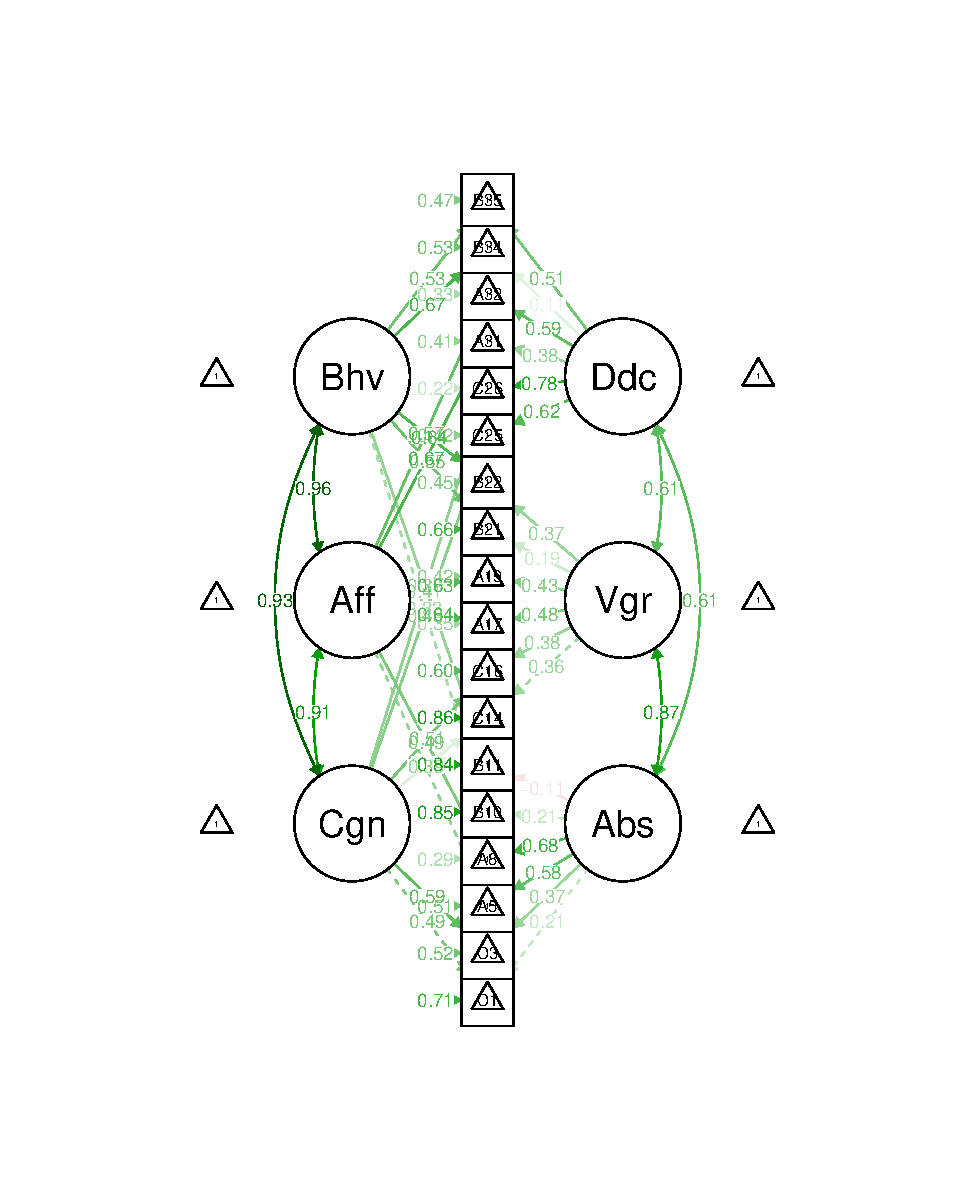
\includegraphics{20to18_files/figure-latex/19to18-1.pdf}
\caption{\label{fig:19to18}Bifactor analysis final 18-item scale(s) definitions.}
\end{figure}

Looking first at the Absorption-Cognition candidate items (1, 3, and 4), Item 4 stood out as a candidate for exclusion based on empirical indices (corrected item-total correlations, inter-item correlations, and bifactor analysis fit; \(\chi^2_{with4}\) = 676.51, \(\chi^2_{without4}\) = 499.05). Conceptually we also agreed that Item 4 was not uniquely critical for comprehensive coverage across either the Cognition or Absorption constructs.

Regarding candidate items 25, 26, and 28, item 25 exhibited the weakest corrected item-total correlation for both Dedication (\emph{r} = .69) and Cognition (\emph{r} = .60), however, the relative magnitudes were moderately high, coefficients for all three items were comparable (ranging from .60 to .78) and the item 25 content was deemed critical for both the Cognition as well as Dedication content domains. Two different CFAs were performed with comparable fit indices - one retaining only item 26 (\(\chi^2_{keep26}\) = 442.39), and the other instead retaining item 28 (\(\chi^2_{keep28}\) = 458.12).

Ultimately the definitional uniqueness of item 26, focusing on percieved reciprocity and support regarding tenure/career objectives led to a decision for retention. This entire scale reduction endeavor, therefore, concluded with the deletions of Item 4, ``I find it difficult to mentally disconnect from work'' and Item 28, ``This organization challenges me to work at my full potential''.

\begin{quote}
Note. Put corrected item-totals table in if have time (for both scales - substantive and attitudinal; probably only items 1, 3, 4 and 25, 26, 28)
\end{quote}

\begin{lltable}

\begin{TableNotes}[para]
\normalsize{\textit{Note.} Items were dropped sequentially, the first two CFAs reflect 19 items and the last two reflect 18}
\end{TableNotes}

\begin{longtable}{llllllll}\noalign{\getlongtablewidth\global\LTcapwidth=\longtablewidth}
\caption{\label{tab:fitindicestable}Fit indices four different bifactor CFAs.}\\
\toprule
Model & \multicolumn{1}{c}{chisq} & \multicolumn{1}{c}{df} & \multicolumn{1}{c}{RMSEA} & \multicolumn{1}{c}{SRMR} & \multicolumn{1}{c}{CFI} & \multicolumn{1}{c}{TLI} & \multicolumn{1}{c}{AIC}\\
\midrule
\endfirsthead
\caption*{\normalfont{Table \ref{tab:fitindicestable} continued}}\\
\toprule
Model & \multicolumn{1}{c}{chisq} & \multicolumn{1}{c}{df} & \multicolumn{1}{c}{RMSEA} & \multicolumn{1}{c}{SRMR} & \multicolumn{1}{c}{CFI} & \multicolumn{1}{c}{TLI} & \multicolumn{1}{c}{AIC}\\
\midrule
\endhead
Original & 676.51 & 145 & 0.06 & 0.04 & 0.94 & 0.93 & 60686.58\\
Retain 1 & 682.6 & 128 & 0.07 & 0.04 & 0.94 & 0.92 & 57744.46\\
Retain 4 & 499.05 & 128 & 0.05 & 0.03 & 0.96 & 0.94 & 57173.78\\
Retain 26 & 442.39 & 112 & 0.05 & 0.03 & 0.96 & 0.94 & 54493.47\\
Retain 28 & 458.12 & 112 & 0.06 & 0.03 & 0.96 & 0.94 & 54425.65\\
\bottomrule
\addlinespace
\insertTableNotes
\end{longtable}

\end{lltable}

\begin{lltable}

\begin{TableNotes}[para]
\normalsize{\textit{Note.} The recommended response scale is 'Strongly Disagree', 'Disagree', 'Somewhat Disagree', 'Somewhat Agree', 'Agree', and 'Strongly Agree'}
\end{TableNotes}

\begin{longtable}{llll}\noalign{\getlongtablewidth\global\LTcapwidth=\longtablewidth}
\caption{\label{tab:itemstable}Suggested final scale definitions.}\\
\toprule
Substantive & \multicolumn{1}{c}{Attitudinal} & \multicolumn{1}{c}{Item.Number} & \multicolumn{1}{c}{Item.Stem}\\
\midrule
\endfirsthead
\caption*{\normalfont{Table \ref{tab:itemstable} continued}}\\
\toprule
Substantive & \multicolumn{1}{c}{Attitudinal} & \multicolumn{1}{c}{Item.Number} & \multicolumn{1}{c}{Item.Stem}\\
\midrule
\endhead
Absorption & Cognitive & 1 & I am able to concentrate on my work without getting distracted\\
Absorption & Cognitive & 3 & Time passes quickly while I'm working\\
Absorption & Affective & 5 & I enjoy thinking about work even when I'm not at work\\
Absorption & Affective & 8 & I love starting my workday\\
Absorption & Behavioral & 10 & I have to be reminded to take breaks while I'm at work\\
Absorption & Behavioral & 11 & I never miss a work deadline\\
Vigor & Cognitive & 14 & Thinking about work saps my energy\\
Vigor & Cognitive & 16 & I'm able to maintain good levels of energy throughout the workday\\
Vigor & Affective & 17 & I enjoy spending time completing my job tasks\\
Vigor & Affective & 19 & I feek motivated to go beyond what is asked of me at work\\
Vigor & Behavioral & 21 & When work is slow I find ways to be productive\\
Vigor & Behavioral & 22 & I express enthusiasm for my job while at work\\
Dedication & Cognitive & 25 & I plan to stay with this company as my career advances\\
Dedication & Cognitive & 26 & I believe this company cares about my career goals\\
Dedication & Affective & 31 & I feel proud of my accomplishments within this organization\\
Dedication & Affective & 32 & My job makes me feel like I'm part of something meaningful\\
Dedication & Behavioral & 34 & I embrace challenging situations at work\\
Dedication & Behavioral & 35 & I speak positively about this organization to others\\
\bottomrule
\addlinespace
\insertTableNotes
\end{longtable}

\end{lltable}

Figure \ref{fig:19to18} presents the visual CFA for the final scale definitions, Table \ref{tab:fitindicestable} presents a more comprehensive table of fit indices, and Table \ref{tab:itemstable} presents the final recommendation regarding the 18-item scale definitions, including the individual item stems.

\hypertarget{discussion}{%
\section{Discussion}\label{discussion}}

We believe that this project has theoretical, methodological, and practical implications. By specifying known sources of item covariance (through \emph{a priori} specification of alternative factors), it is possible that we may help explain some of the high inter-scale correlations that have been reported with other measures of engagement. We do this via extension of the bifactor analsis tradition, which historically has been used in common method variance investigations where only ``one'' alternative factor is specified. Although not common in the literature, we hope that this type of extension of bifactor analyses may be further pursued and investigated.

Our primary aspiration for developing this measure was that it would be a public domain instrument that would draw equal appeal from both practitioners and academics. These preliminary investigations suggest that it is scalable to two aggregations which we have been referring to as: 1) research (DAC), and 2) actionable (ABC). Our (as-of-yet untested) assumption is that practitioners may be more interested in feedback regarding how their employees \emph{think}, \emph{feel}, and \emph{behave} with regard to engagement. Academics, on the other hand, may be more interested in possible differentiation between levels of dedication, absorption, and vigor. Having one assessment that may aggregate to either framework not only addresses the demand of constituent users, but it also facilitates aggregation across samplings for broader purposes such as norms development, validation, and metaanalysis.

\newpage

\hypertarget{references}{%
\section{References}\label{references}}

\hypertarget{refs}{}
\begin{CSLReferences}{1}{0}
\leavevmode\vadjust pre{\hypertarget{ref-R-papaja}{}}%
Aust, F., \& Barth, M. (2022). \emph{{papaja}: {Prepare} reproducible {APA} journal articles with {R Markdown}}. \url{https://github.com/crsh/papaja}

\leavevmode\vadjust pre{\hypertarget{ref-towersperrin2009}{}}%
Ballendowitsch, J., \& Perrin-ISR, T. (2009). Employee engagement--a way forward to productivity. \emph{Towers Perrin-ISR Case Study, Towers Perrin-ISR}, \emph{14}.

\leavevmode\vadjust pre{\hypertarget{ref-R-tinylabels}{}}%
Barth, M. (2022). \emph{{tinylabels}: Lightweight variable labels}. \url{https://cran.r-project.org/package=tinylabels}

\leavevmode\vadjust pre{\hypertarget{ref-baumruk2004missing}{}}%
Baumruk, R. (2004). \emph{The missing link: The role of employee engagement in business success}. \emph{47}, 48--52.

\leavevmode\vadjust pre{\hypertarget{ref-biderman2011ubiquity}{}}%
Biderman, M. D., Nguyen, N. T., Cunningham, C. J., \& Ghorbani, N. (2011). The ubiquity of common method variance: The case of the big five. \emph{Journal of Research in Personality}, \emph{45}(5), 417--429.

\leavevmode\vadjust pre{\hypertarget{ref-blessingwhite2018}{}}%
BlessingWhite. (2018). \emph{Employee engagement survey}. Available at \url{https://blessingwhite.com/wp-content/uploads/2019/11/Employee_Engagement_Survey_Fact_Sheet.pdf}.

\leavevmode\vadjust pre{\hypertarget{ref-coffman_hard_1999}{}}%
Coffman, C., \& Harter, J. (1999). A hard look at soft numbers. \emph{Position Paper, Gallup Organization}.

\leavevmode\vadjust pre{\hypertarget{ref-cole2012job}{}}%
Cole, M. S., Walter, F., Bedeian, A. G., \& O'Boyle, E. H. (2012). Job burnout and employee engagement: A meta-analytic examination of construct proliferation. \emph{Journal of Management}, \emph{38}(5), 1550--1581.

\leavevmode\vadjust pre{\hypertarget{ref-csikszentmihalyi1990flow}{}}%
Csikszentmihalyi, M. (1990). \emph{Flow: The psychology of optimal experience} (Vol. 1990). Harper \& Row New York.

\leavevmode\vadjust pre{\hypertarget{ref-R-descr}{}}%
Dirk Enzmann, J. Aquino. I. R. source code and/or documentation written by, Schwartz, M., Jain, N., \& Kraft, S. (2021). \emph{Descr: Descriptive statistics}. \url{https://CRAN.R-project.org/package=descr}

\leavevmode\vadjust pre{\hypertarget{ref-elloy_examination_1991}{}}%
Elloy, D. F., Everett, J. E., \& Flynn, W. R. (1991). An examination of the correlates of job involvement. \emph{Group \& Organization Studies}, \emph{16}(2), 160--177. \url{https://doi.org/10.1177/105960119101600204}

\leavevmode\vadjust pre{\hypertarget{ref-ferris_added_1984}{}}%
Ferris, R., \& Hellier, P. (1984). Added value productivity schemes and employee participation. \emph{Asia Pacific Journal of Human Resources}, \emph{22}(4), 35--44. \url{https://doi.org/10.1177/103841118402200406}

\leavevmode\vadjust pre{\hypertarget{ref-gade2017disentangling}{}}%
Gäde, J. C., Schermelleh-Engel, K., \& Klein, A. G. (2017). Disentangling the common variance of perfectionistic strivings and perfectionistic concerns: A bifactor model of perfectionism. \emph{Frontiers in Psychology}, \emph{8}, 160.

\leavevmode\vadjust pre{\hypertarget{ref-giordano_exploratory_2020}{}}%
Giordano, C., Ones, D. S., Waller, N. G., \& Stanek, K. C. (2020). Exploratory bifactor measurement models in vocational behavior research. \emph{Journal of Vocational Behavior}, \emph{120}, 103430. \url{https://doi.org/10.1016/j.jvb.2020.103430}

\leavevmode\vadjust pre{\hypertarget{ref-goering2017not}{}}%
Goering, D. D., Shimazu, A., Zhou, F., Wada, T., \& Sakai, R. (2017). Not if, but how they differ: A meta-analytic test of the nomological networks of burnout and engagement. \emph{Burnout Research}, \emph{5}, 21--34.

\leavevmode\vadjust pre{\hypertarget{ref-harter_relationship_2013}{}}%
Harter, J. K., Schmidt, F. L., Agrawal, S., \& Plowman, S. K. (2013). The relationship between engagement at work and organizational outcomes 2012 Q12 meta-analysis lincoln. \emph{{NE}: The Gallup Organization}.

\leavevmode\vadjust pre{\hypertarget{ref-hewitt2017}{}}%
Hewitt, A. (2017). \emph{2017 trends in global employee engagement}. Available at \url{https://content.lesaffaires.com/LAF/lacom/Aon_2017_Employee-Engagement.pdf}.

\leavevmode\vadjust pre{\hypertarget{ref-kahn1990psychological}{}}%
Kahn, W. A. (1990a). Psychological conditions of personal engagement and disengagement at work. \emph{Academy of Management Journal}, \emph{33}(4), 692--724.

\leavevmode\vadjust pre{\hypertarget{ref-kahn_psychological_1990}{}}%
Kahn, W. A. (1990b). Psychological conditions of personal engagement and disengagement at work. \emph{Academy of Management Journal}, \emph{33}(4), 692--724.

\leavevmode\vadjust pre{\hypertarget{ref-kaiser_campbell_2019}{}}%
Kaiser, F. G., \& Wilson, M. (2019). The {Campbell} {Paradigm} as a {Behavior}-{Predictive} {Reinterpretation} of the {Classical} {Tripartite} {Model} of {Attitudes}. \emph{European Psychologist}, \emph{24}(4), 359--374. \url{https://doi.org/10.1027/1016-9040/a000364}

\leavevmode\vadjust pre{\hypertarget{ref-kim_burnout_2009}{}}%
Kim, H. J., Shin, K. H., \& Swanger, N. (2009). Burnout and engagement: {A} comparative analysis using the {Big} {Five} personality dimensions. \emph{International Journal of Hospitality Management}, \emph{28}(1), 96--104. \url{https://doi.org/10.1016/j.ijhm.2008.06.001}

\leavevmode\vadjust pre{\hypertarget{ref-leiter_areas_2004}{}}%
Leiter, M., \& Maslach, C. (2004). Areas of worklife: A structured approach to organizational predictors of job burnout. In \emph{Research in occupational stress and well-being} (Vol. 3, pp. 91--134). \url{https://doi.org/10.1016/S1479-3555(03)03003-8}

\leavevmode\vadjust pre{\hypertarget{ref-leone_relation_1995}{}}%
Leone, D. R. (1995). \emph{The relation of work climate, higher order need satisfaction, need salience, and causality orientations to work engagement, psychological adjustment, and job satisfaction} {[}PhD thesis{]}. ProQuest Information \& Learning.

\leavevmode\vadjust pre{\hypertarget{ref-maslach1997causes}{}}%
Maslach, C., \& Leiter, M. (1997). What causes burnout. \emph{Maslach C, Leiter MP. The Truth About Burnout: How Organizations Cause Personal Stress and What to Do about It. San Francisco, CA: Josey-Bass Publishers}, 38--60.

\leavevmode\vadjust pre{\hypertarget{ref-maslach_early_2008}{}}%
Maslach, C., \& Leiter, M. P. (2008). Early predictors of job burnout and engagement. \emph{Journal of Applied Psychology}, \emph{93}(3), 498--512.

\leavevmode\vadjust pre{\hypertarget{ref-meyer_three-component_1991}{}}%
Meyer, J. P., \& Allen, N. J. (1991). A three-component conceptualization of organizational commitment. \emph{Human Resource Management Review}, \emph{1}(1), 61--89.

\leavevmode\vadjust pre{\hypertarget{ref-R-base}{}}%
R Core Team. (2022). \emph{R: A language and environment for statistical computing}. R Foundation for Statistical Computing. \url{https://www.R-project.org/}

\leavevmode\vadjust pre{\hypertarget{ref-reise_rediscovery_2012}{}}%
Reise, S. P. (2012). The rediscovery of bifactor measurement models. \emph{Multivariate Behavioral Research}, \emph{47}(5), 667--696. \url{https://doi.org/10.1080/00273171.2012.715555}

\leavevmode\vadjust pre{\hypertarget{ref-rosenberg_cognitive_1960}{}}%
Rosenberg, M. J. (1960). Cognitive, affective, and behavioral components of attitudes. In \emph{Attitude organization and change}.

\leavevmode\vadjust pre{\hypertarget{ref-R-lavaan}{}}%
Rosseel, Y. (2012). {lavaan}: An {R} package for structural equation modeling. \emph{Journal of Statistical Software}, \emph{48}(2), 1--36. \url{https://doi.org/10.18637/jss.v048.i02}

\leavevmode\vadjust pre{\hypertarget{ref-engage_2022}{}}%
Russell, M., Ossorio Duffoo, C., Garcia Prieto Palacios Roji, R., \& Kulas, J. (2022). Development of an intentional bifactor measure of engagement. \emph{The Seattle Edition of SIOP}, 1--14.

\leavevmode\vadjust pre{\hypertarget{ref-saks_antecedents_2006}{}}%
Saks, A. M. (2006). Antecedents and consequences of employee engagement. \emph{Journal of Managerial Psychology}.

\leavevmode\vadjust pre{\hypertarget{ref-saks2019antecedents}{}}%
Saks, A. M. (2019). Antecedents and consequences of employee engagement revisited. \emph{Journal of Organizational Effectiveness: People and Performance}, \emph{6}(1), 19--38.

\leavevmode\vadjust pre{\hypertarget{ref-schaufeli2013engagement}{}}%
Schaufeli, W. B. (2013). What is engagement? In \emph{Employee engagement in theory and practice} (pp. 29--49). Routledge.

\leavevmode\vadjust pre{\hypertarget{ref-schaufeli_uwesutrecht_2003}{}}%
Schaufeli, W. B., \& Bakker, A. B. (2003). {UWES}--utrecht work engagement scale: Test manual. \emph{Unpublished Manuscript: Department of Psychology, Utrecht University}, \emph{8}.

\leavevmode\vadjust pre{\hypertarget{ref-schaufeli_measurement_2002}{}}%
Schaufeli, W. B., Salanova, M., González-Romá, V., \& Bakker, A. B. (2002). The measurement of engagement and burnout: A two sample confirmatory factor analytic approach. \emph{Journal of Happiness Studies}, \emph{3}(1), 71--92.

\leavevmode\vadjust pre{\hypertarget{ref-schaufeli2008workaholism}{}}%
Schaufeli, W. B., Taris, T. W., \& Van Rhenen, W. (2008). Workaholism, burnout, and work engagement: Three of a kind or three different kinds of employee well-being? \emph{Applied Psychology}, \emph{57}(2), 173--203.

\leavevmode\vadjust pre{\hypertarget{ref-schaufeli_conceptualization_2010}{}}%
Schaufeli, W., \& Bakker, A. (2010). The conceptualization and measurement of work engagement. In W. Schaufeli, A. Bakker, \& M. Leiter (Eds.), \emph{Work engagement: A handbook of essential theory and research} (pp. 10--24). Psychology Press.

\leavevmode\vadjust pre{\hypertarget{ref-shaw2005engagement}{}}%
Shaw, K. (2005). An engagement strategy process for communicators. \emph{Strategic Communication Management}, \emph{9}(3), 26.

\leavevmode\vadjust pre{\hypertarget{ref-sirota2013enthusiastic}{}}%
Sirota, D., \& Klein, D. (2013). \emph{The enthusiastic employee: How companies profit by giving workers what they want}. FT Press.

\leavevmode\vadjust pre{\hypertarget{ref-soane2012development}{}}%
Soane, E., Truss, C., Alfes, K., Shantz, A., Rees, C., \& Gatenby, M. (2012). Development and application of a new measure of employee engagement: The ISA engagement scale. \emph{Human Resource Development International}, \emph{15}(5), 529--547.

\leavevmode\vadjust pre{\hypertarget{ref-staw_employee_1994}{}}%
Staw, B. M., Sutton, R. I., \& Pelled, L. H. (1994). Employee positive emotion and favorable outcomes at the workplace. \emph{Organization Science}, \emph{5}(1), 51--71.

\leavevmode\vadjust pre{\hypertarget{ref-taris2017burnout}{}}%
Taris, T. W., Ybema, J. F., \& Beek, I. van. (2017). Burnout and engagement: Identical twins or just close relatives? \emph{Burnout Research}, \emph{5}, 3--11.

\leavevmode\vadjust pre{\hypertarget{ref-timms2012burnt}{}}%
Timms, C., Brough, P., \& Graham, D. (2012). Burnt-out but engaged: The co-existence of psychological burnout and engagement. \emph{Journal of Educational Administration}, \emph{50}(3), 327--345.

\leavevmode\vadjust pre{\hypertarget{ref-trogolo2020work}{}}%
Trógolo, M. A., Morera, L. P., Castellano, E., Spontón, C., \& Medrano, L. A. (2020). Work engagement and burnout: Real, redundant, or both? A further examination using a bifactor modelling approach. \emph{European Journal of Work and Organizational Psychology}, \emph{29}(6), 922--937.

\leavevmode\vadjust pre{\hypertarget{ref-R-careless}{}}%
Yentes, R. D., \& Wilhelm, F. (2021). \emph{Careless: Procedures for computing indices of careless responding}.

\end{CSLReferences}


\end{document}
